\ifnum \Version=1  
\question[2] Consider the autonomous differential equation $\displaystyle \frac{dy}{dt}= (y-1)(y-k^2)$.  Assume $k$ can be any real number. Draw the bifurcation diagram on the axes below. That is, plot the location of the critical points versus $k$. Please label your axes.
        \begin{center}
        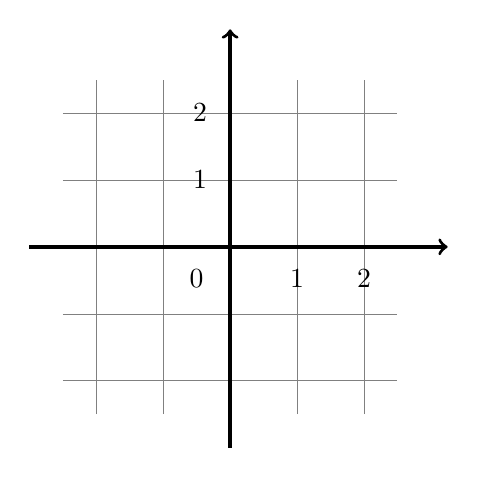
\begin{tikzpicture}[scale=0.85]
        \draw[help lines] (-2.5,-2.5) grid (2.5, 2.5);
        \draw[very thick, ->] (-3, 0) -- (3.25, 0);
        \draw[very thick, ->] (0, -3) -- (0, 3.25);
        \node[overlay, left] at (-0.2, 1) {$1$};
        \node[overlay, left] at (-0.2, 2) {$2$};
        \node[overlay, below] at (-0.5, -0.2) {$0$};
        \node[overlay, below] at (1, -0.2) {$1$};
        \node[overlay, below] at (2, -0.2) {$2$};
        \end{tikzpicture}
        \end{center}
\fi

\ifnum \Version=2
\question[2] Consider the autonomous differential equation $\displaystyle \frac{dy}{dt}= (y-k)(y+1-k^2)$.  Assume $k$ can be any real number. Draw the bifurcation diagram on the axes below. That is, plot the location of the critical points versus $k$. Please label your axes.
        \begin{center}
        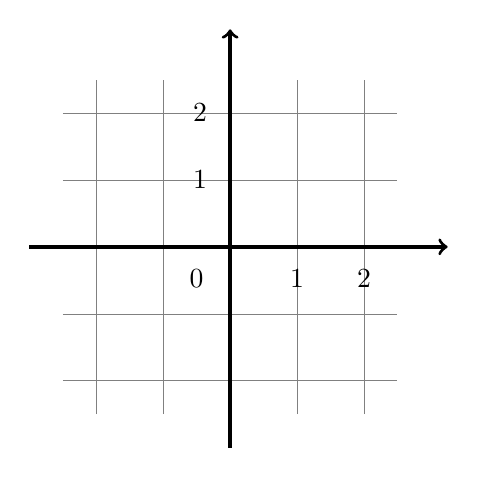
\begin{tikzpicture}[scale=0.85]
        \draw[help lines] (-2.5,-2.5) grid (2.5, 2.5);
        \draw[very thick, ->] (-3, 0) -- (3.25, 0);
        \draw[very thick, ->] (0, -3) -- (0, 3.25);
        \node[overlay, left] at (-0.2, 1) {$1$};
        \node[overlay, left] at (-0.2, 2) {$2$};
        \node[overlay, below] at (-0.5, -0.2) {$0$};
        \node[overlay, below] at (1, -0.2) {$1$};
        \node[overlay, below] at (2, -0.2) {$2$};
        \end{tikzpicture}
        \end{center}
\fi

\ifnum \Version=3
    \question[2] You do not need to show your work for this question. Consider the differential equation 
    \begin{align*}
        t^2y'' - 4ty' - 2y = 12
    \end{align*}
    The DE can be expressed in the form $\vec x\, ' = A\vec x + \vec g$, where 
    \begin{align*}
     A = \left( \hbox to 2cm{\vbox to 0.85cm{}} \right), \quad \vec g = \left( \hbox to 1.2cm{\vbox to 0.85cm{}} \right)
    \end{align*}
    Fill in the missing entries in the above to define $A$ and $\vec g$. 
\fi

\ifnum \Version=4
\question[2] Consider the autonomous differential equation $\displaystyle \frac{dy}{dt}= (y+k)(y^2-k)$.  Assume $k\ge0$. Draw the bifurcation diagram on the axes below. That is, plot the location of the critical points versus $k$. Please label your axes.
        \begin{center}
        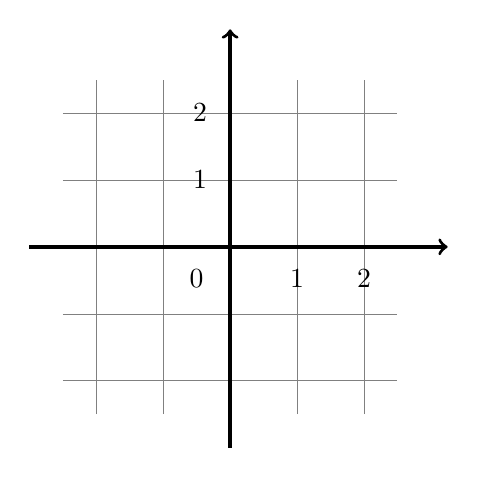
\begin{tikzpicture}[scale=0.85]
        \draw[help lines] (-2.5,-2.5) grid (2.5, 2.5);
        \draw[very thick, ->] (-3, 0) -- (3.25, 0);
        \draw[very thick, ->] (0, -3) -- (0, 3.25);
        \node[overlay, left] at (-0.2, 1) {$1$};
        \node[overlay, left] at (-0.2, 2) {$2$};
        \node[overlay, below] at (-0.5, -0.2) {$0$};
        \node[overlay, below] at (1, -0.2) {$1$};
        \node[overlay, below] at (2, -0.2) {$2$};
        \end{tikzpicture}
        \end{center}
\fi

\ifnum \Version=5
    \question[2] You do not need to show your work for this question. Consider the differential equation 
    \begin{align*}
        4y'' - t^2y' - 2ty = 12\cos(t)
    \end{align*}
    The DE can be expressed in the form $\vec x\, ' = A\vec x + \vec g$, where 
    \begin{align*}
     A = \left( \hbox to 2cm{\vbox to 0.85cm{}} \right), \quad \vec g = \left( \hbox to 1.2cm{\vbox to 0.85cm{}} \right)
    \end{align*}
    Fill in the missing entries in the above to define $A$ and $\vec g$. 
\fi




\ifnum \Version=6
\question[1] You do not need to show your work for this question. Consider the IVP below.
$$\displaystyle y' = \sqrt{4-t^2+y}, \ y(1) = 2$$   
Using the theorems we covered in lecture, fill in all of the appropriate circles below to indicate the intervals over which there must contain a unique solution to the IVP. 
\begin{itemize}
    \item[$\bigcirc$] $y \ge 4-t^2$
    \item[$\bigcirc$] $y \le 4-t^2$
    \item[$\bigcirc$] $y \le t^2-4$
    \item[$\bigcirc$] $y \ge t^2-4$
    \item[$\bigcirc$] none of the above
\end{itemize}
\ifnum \Solutions=1 {\color{DarkBlue} 
\textbf{Solutions:} the relevant theorem is below. 

    \begin{center}\begin{tikzpicture} \node [mybox](box){\begin{minipage}{0.95\textwidth} \vspace{4pt}

    If $f$ and $\frac{\partial f}{\partial y}$ are continuous over $\alpha < t < \beta$, and $\gamma < y < \delta$, which contains the point $(t_0,y_0)$, then there is a unique solution to the IVP $$y' = f(t,y), \quad y(t_0) = y_0$$ on an interval contained in $\alpha < t < \beta$. 
    
    \end{minipage}}; \node[fancytitle, rounded corners, thick, inner sep = 4pt, right=10pt] at (box.north west) {Theorem 2.4.2: Existence and Uniqueness of 1st Order Nonlinear IVP};
    \end{tikzpicture}\end{center}
    
    Taking the partial derivative with respect to $y$:
\begin{align}
    \frac{\partial f}{\partial y} &= \frac{1}{\sqrt{4-t^2+y}}\\
\end{align}
The relevant functions are 
\begin{align}
    f(t,y) &= \sqrt{4-t^2+y} \\
    \frac{\partial f}{\partial y} &= \frac{1}{\sqrt{4-t^2+y}}
\end{align}
They are real and continuous over $$4-t^2+y > 0$$ and this interval also contains $t_0 = 0$ and $y(t_0)$. So the interval over which there must contain a unique solution is $$y > t^2-4$$ 
} 
\else 
\fi
\fi 




\ifnum \Version=7
\question[1] You do not need to show your work for this question. Consider the IVP below.
$$\displaystyle (t+3)y' + \sqrt{4-t^2}\,y = t^4, \ y(1) = 9$$   
Using the theorems we covered in lecture, fill in all of the appropriate circles below to indicate the intervals over which there must contain a unique solution to the IVP. 
\begin{itemize}
    \item[$\bigcirc$] $-3 < t \le 2$
    \item[$\bigcirc$] $-2 \le t \le 2$
    \item[$\bigcirc$] $-2 \le t \le 3$    
    \item[$\bigcirc$] $-\infty \le t < -3$
    \item[$\bigcirc$] none of the above
\end{itemize}
\ifnum \Solutions=1 {\color{DarkBlue} 
\textbf{Solutions:} convert to standard form:
\begin{align}
    y' + \frac{\sqrt{4-t^2}}{t+3}\,y = \frac{t^4}{t+3}
\end{align}
The coefficients are real and continuous over $$-2\le t \le 2$$ and this interval also contains $t_0 = 1$. So the interval over which there must contain a unique solution is $-2\le t \le 2$. 
} 
\else 
\fi
\fi 



\ifnum \Version=8
\question[1] You do not need to show your work for this question. Consider the IVP below.
$$\displaystyle y' = \sqrt{4-t^2-y}, \ y(0) = 2$$   
Using the theorems we covered in lecture, fill in all of the appropriate circles below to indicate the intervals over which there must contain a unique solution to the IVP. 
\begin{itemize}
    \item[$\bigcirc$] $y \ge 4-t^2$
    \item[$\bigcirc$] $y \le 4-t^2$
    \item[$\bigcirc$] $y \le t^2-4$
    \item[$\bigcirc$] $y \ge t^2-4$
    \item[$\bigcirc$] none of the above
\end{itemize}
\ifnum \Solutions=1 {\color{DarkBlue} 
\textbf{Solutions:} partial derivative with respect to $y$:
\begin{align}
    \frac{\partial f}{\partial y} &= \frac{-1}{\sqrt{4-t^2-y}}
\end{align}
The coefficients are real and continuous over $$4-t^2-y\ge 0$$ and this interval also contains $t_0 = 0$ and $y(t_0)$. So the interval over which there must contain a unique solution is $y \le 4-t^2$. 
} 
\else 
\fi
\fi 



\ifnum \Version=9
\question[1] You do not need to show your work for this question. Consider the IVP below.
$$\displaystyle y' = \sqrt{4-t^2+y}, \ y(0) = 2$$   
Using the theorems we covered in lecture, fill in all of the appropriate circles below to indicate the intervals over which there must contain a unique solution to the IVP. 
\begin{itemize}
    \item[$\bigcirc$] $y \ge 4-t^2$
    \item[$\bigcirc$] $y \le 4-t^2$
    \item[$\bigcirc$] $y \le t^2-4$
    \item[$\bigcirc$] $y \ge t^2-4$
    \item[$\bigcirc$] none of the above
\end{itemize}
\ifnum \Solutions=1 {\color{DarkBlue} 
\textbf{Solutions:} partial derivative with respect to $y$:
\begin{align}
    \frac{\partial f}{\partial y} &= \frac{1}{\sqrt{4-t^2+y}}\\
\end{align}
The coefficients are real and continuous over $$4-t^2+y\ge 0$$ and this interval also contains $t_0 = 0$ and $y(t_0)$. So the interval over which there must contain a unique solution is $y \ge t^2-4$. 
} 
\else 
\fi
\fi 



